%%%%%%%%%%%%%%%%%%%%%%%%%%%%%%%%%%%%%%%%%
% a0poster Landscape Poster
% LaTeX Template
% Version 1.0 (22/06/13)
%
% The a0poster class was created by:
% Gerlinde Kettl and Matthias Weiser (tex@kettl.de)
% 
% This template has been downloaded from:
% http://www.LaTeXTemplates.com
%
% License:
% CC BY-NC-SA 3.0 (http://creativecommons.org/licenses/by-nc-sa/3.0/)
%
%%%%%%%%%%%%%%%%%%%%%%%%%%%%%%%%%%%%%%%%%

%----------------------------------------------------------------------------------------
%	PACKAGES AND OTHER DOCUMENT CONFIGURATIONS
%----------------------------------------------------------------------------------------

\documentclass[a0,landscape,beamer]{a0poster}

\usepackage{multicol} % This is so we can have multiple columns of text side-by-side
\columnsep=100pt % This is the amount of white space between the columns in the poster
\columnseprule=3pt % This is the thickness of the black line between the columns in the poster

\usepackage[svgnames]{xcolor} % Specify colors by their 'svgnames', for a full list of all colors available see here: http://www.latextemplates.com/svgnames-colors

\usepackage{times} % Use the times font
%\usepackage{palatino} % Uncomment to use the Palatino font
\usepackage{float}
\usepackage{graphicx} % Required for including images
\graphicspath{{figures/}} % Location of the graphics files
\usepackage{booktabs} % Top and bottom rules for table
\usepackage[font=small,labelfont=bf]{caption} % Required for specifying captions to tables and figures
\usepackage{amsfonts, amsmath, amsthm, amssymb} % For math fonts, symbols and environments
\usepackage{wrapfig} % Allows wrapping text around tables and figures
\usepackage{multirow}
\restylefloat{table}

\begin{document}

%----------------------------------------------------------------------------------------
%	POSTER HEADER 
%----------------------------------------------------------------------------------------

% The header is divided into three boxes:
% The first is 55% wide and houses the title, subtitle, names and university/organization
% The second is 25% wide and houses contact information
% The third is 19% wide and houses a logo for your university/organization or a photo of you
% The widths of these boxes can be easily edited to accommodate your content as you see fit

\begin{minipage}[b]{0.8\linewidth}
\veryHuge \color{NavyBlue} \textbf{Strength in numbers? Modelling the impact of businesses on each other} \color{Black}\\ % Title
\Huge\textit{An exploration of the Yelp dataset}\\[1cm] % Subtitle
\huge \textbf{Amir Sadeghian \& Hakan Inan \& Andres N\"otzli}\\ % Author(s)
\huge PhD Students, Stanford University\\ % University/organization
\end{minipage}
%
\begin{minipage}[t]{0.2\linewidth}

\includegraphics[width=12cm]{logo.png} % Logo or a photo of you, adjust its dimensions here
\end{minipage}

\vspace{1cm} % A bit of extra whitespace between the header and poster content

%----------------------------------------------------------------------------------------

\begin{multicols}{4} % This is how many columns your poster will be broken into, a poster with many figures may benefit from less columns whereas a text-heavy poster benefits from more

%----------------------------------------------------------------------------------------
%	INTRODUCTION
%----------------------------------------------------------------------------------------

\color{SaddleBrown} % SaddleBrown color for the introduction

\section*{Introduction}
In many cities, there is a small number of streets with a lot of restaurants. Being in a street like this is a double-edged sword for the individual restaurant. On one side, it is valuable because it gets them the attention of potential customers for free. On the other hand, the restaurants are competing for customers with similar needs and the offerings are not free from overlap. When a new business opens in a cluster, this delicate balance is disturbed. The goal of this project is to model the impact of a new business on the existing businesses.
Our hypothesis is that the new business has an impact on the perception of customers of existing businesses.
With increased competition, customers have to reevaluate existing businesses taking into account the new options.
We use customer ratings as a proxy for the value of a business and to observe this reevaluation.

%----------------------------------------------------------------------------------------
%	OBJECTIVES
%----------------------------------------------------------------------------------------
\color{Navy} % Navy color for the abstract

\section*{Main Objectives}
\begin{enumerate}
\item Business Clustering
\item Impact of a new business on a cluster
	\begin{itemize}
 	 \item Propose and test impact models
 	 \item Use machine learning techniques to predict the impact
  	\end{itemize}
	
\end{enumerate}


\color{DarkSlateGray} % DarkSlateGray color for the rest of the content

%----------------------------------------------------------------------------------------
%	MATERIALS AND METHODS
%----------------------------------------------------------------------------------------

\section*{Dataset}
Yelp is a website where users view and review businesses like restaurants. The dataset contains data from several cities and there is a rich set of attributes for each business. \\

\begin{minipage}[b]{0.45\linewidth}
\begin{itemize}
	\item[
\includegraphics{Yelp_logo.png}]42,153 businesses 
	\item[
\includegraphics{Yelp_logo.png}] 320,002 business attr.
    \item[
\includegraphics{Yelp_logo.png}] 31,617 check-in sets 
\end{itemize}
\end{minipage}
\begin{minipage}[b]{0.45\linewidth}
\begin{itemize}
    \item[
\includegraphics{Yelp_logo.png}] 252,898 users
    \item[
\includegraphics{Yelp_logo.png}] 403,210 tips 
    \item[
\includegraphics{Yelp_logo.png}] 1,125,458 reviews
\end{itemize}
\end{minipage}



%----------------------------------------------------------------------------------------
%	Preprocessing 
%----------------------------------------------------------------------------------------
\section*{Preprocessing}
\subsection*{Running average of ratings}
The running average of ratings plays an important role when predicting the correlation of two businesses.
The raw user ratings are highly noisy and relatively sparse.
Figure~\ref{fig:moving_average} depicts an example of a moving average for a business over time.
In addition, we filter out businesses with a low number of ratings.

\begin{center}\vspace{1cm}
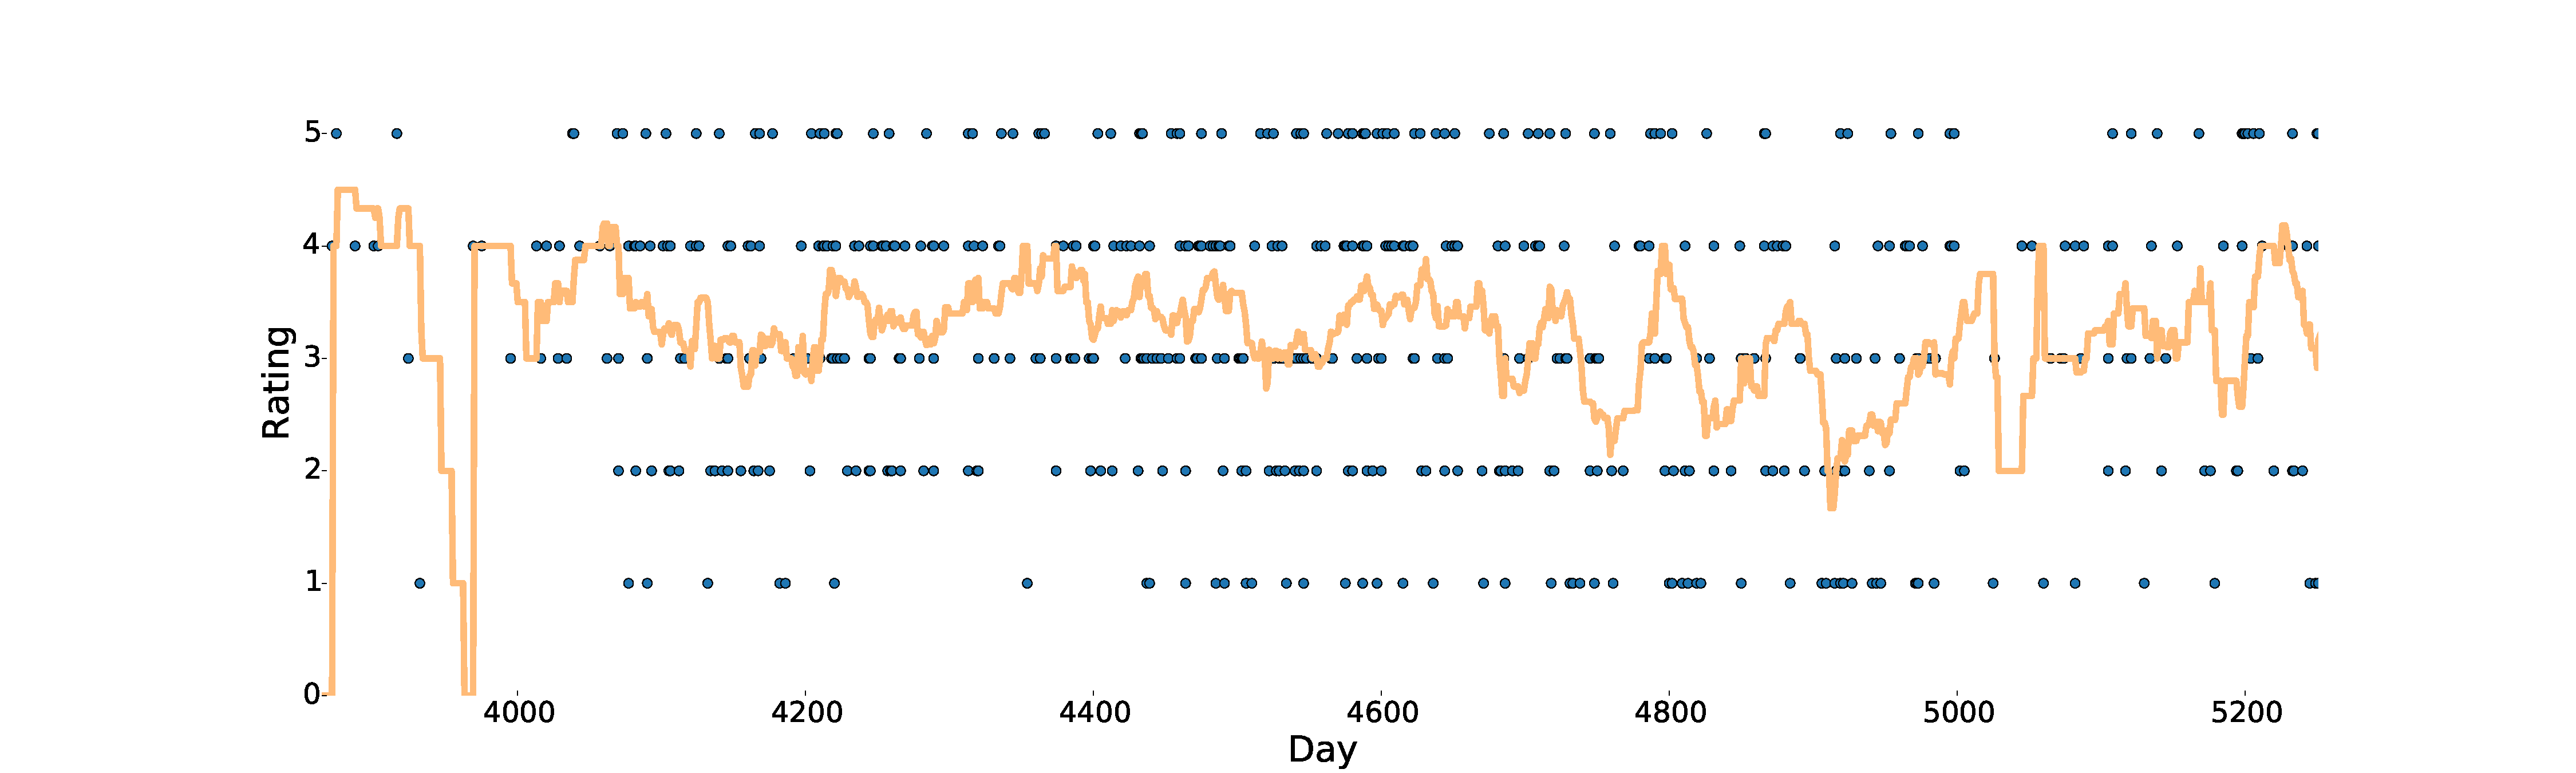
\includegraphics[width=1\linewidth]{../moving_avg.pdf}
\captionof{figure}{\color{Green} Moving average of ratings for a specific business}
\label{fig:moving_average}
\end{center}\vspace{1cm}
 

\subsection*{Business Clustering}
We checked different clustering algorithms and for the same number of clusters, K-Means based on the geographic locations of businesses had the best result. The result of two clustering algorithms results are shown in Figure~\ref{fig:clusters}.
\begin{center}\vspace{1cm}
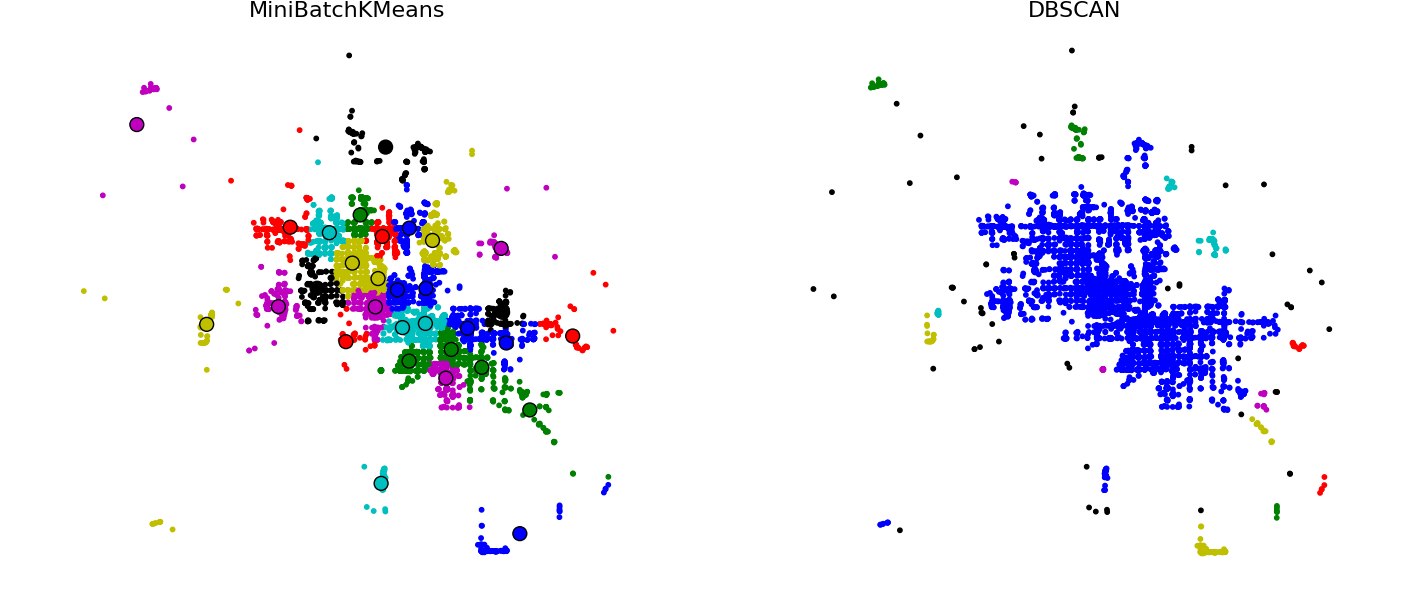
\includegraphics[width=1\linewidth]{clusters.png}
\captionof{figure}{\color{Green} K-Means and DBSCAN clustering}
\label{fig:clusters}
\end{center}\vspace{1cm}

%------------------------------------------------

\section*{Models}

\subsection*{Features}
We found that a combination of geographical distance, price range difference, age, and business categories work best as features to describe the relationship between two businesses. The categories encode attributes of a restaurant like the type of food that it serves.

\subsection*{Conditional Mean Analysis}
\textbf{\textit{Hypothesis}} : Opening of a new business has an impact on the mean of ratings of the  businesses nearby.\\
\textbf{\textit{Proxy}} : Calculate the mean ratings of the nearby businesses before and after a new business opens, and get a comparative metric.\\
\textbf{\textit{Expected results}} : The change in the conditional means of the existing businesses may be predicted using the attributes of the existing businesses and the new business. 

\begin{small}
\begin{align*}
E_{before}(b)=\frac{1}{R_b} \sum_{x: -M+d_0\le d_x \le d_0} r_x(b)\hspace{10mm} & E_{after}(b)=\frac{1}{R_a} \sum_{x: d_0\le d_x \le d_0+M} r_x(b),\\ \\
d_x = \small\text{day of the review x } \hspace{10mm} &d_0 = \small\text{opening day of the new business} \\
 r_x = \small\text{rating of review x}  \hspace{10mm} &M = \small\text{number of days to average over}
\label{eqn:condMean}
\end{align*}
\end{small}
\begin{center}
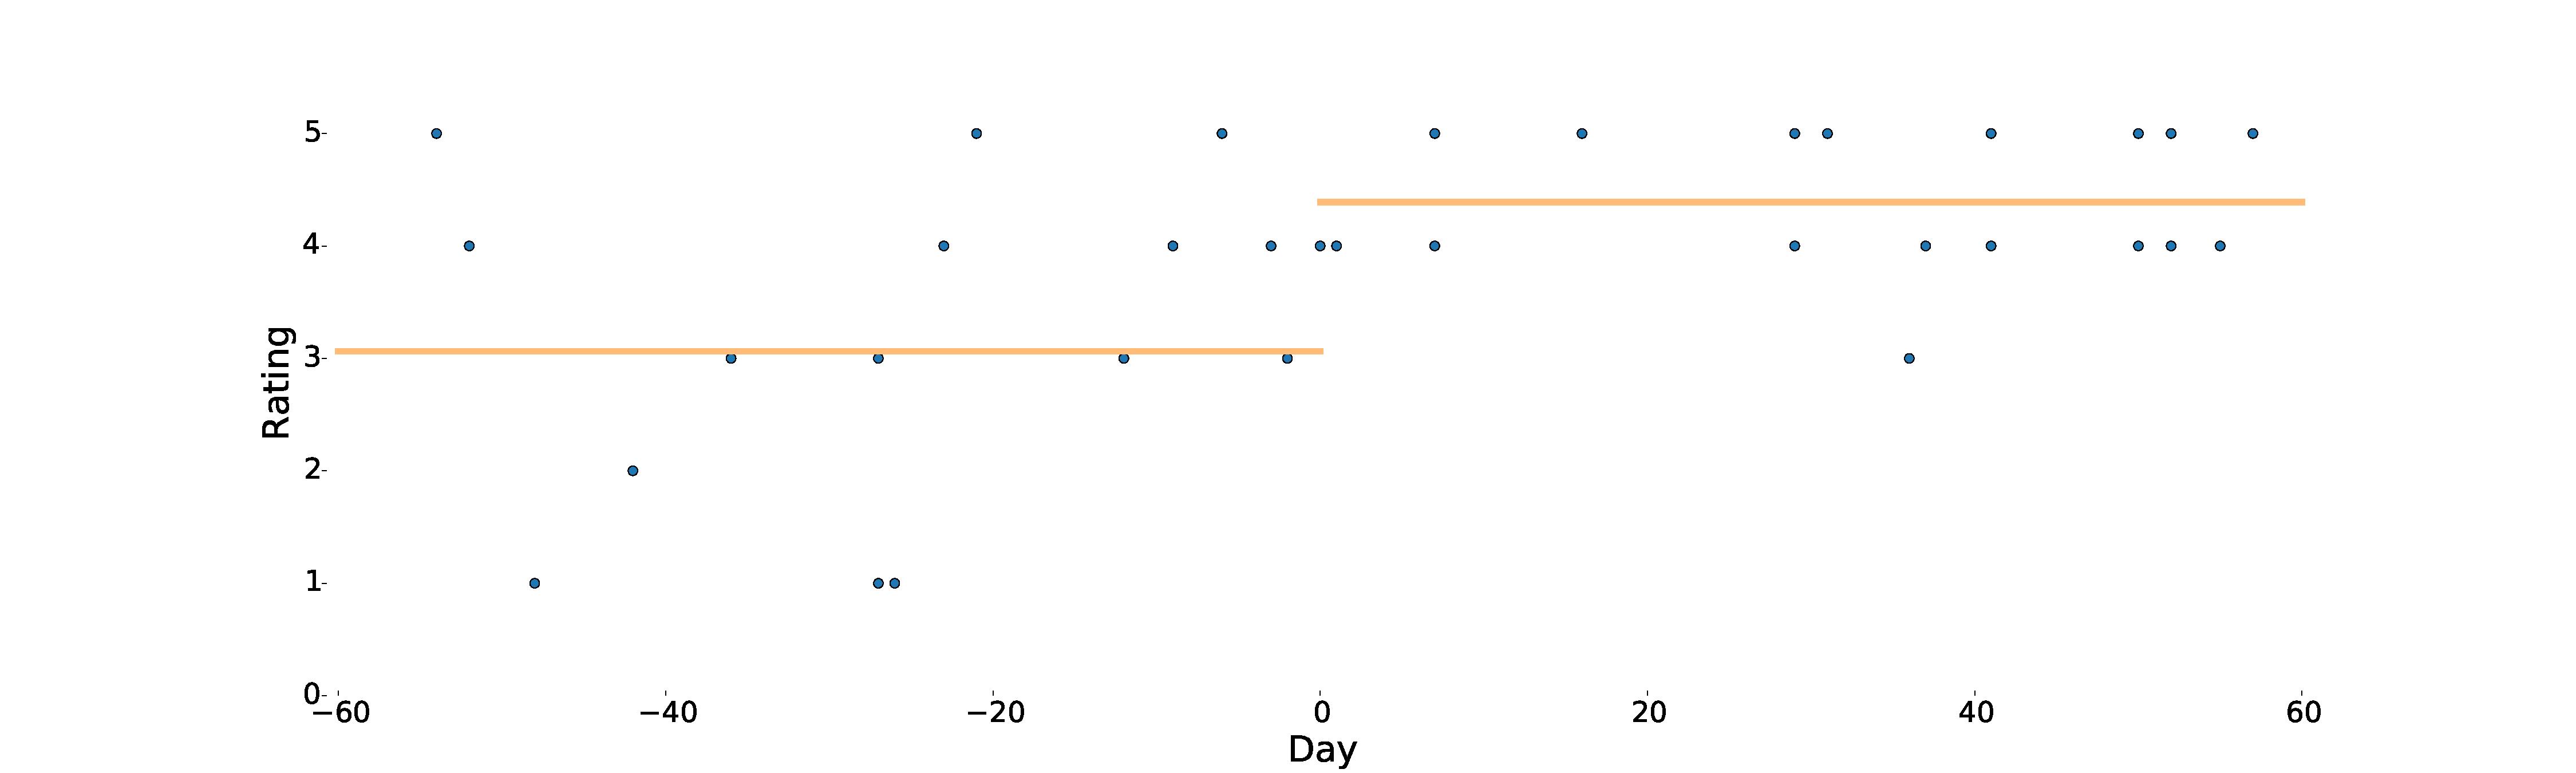
\includegraphics[width=\linewidth]{../mean.pdf}
\captionof{figure}{\color{Green} Example mean analysis for a pair of businesses}
\end{center}

\subsection*{Trend Analysis}
\textbf{\textit{Hypothesis}} : Opening of a new business has an impact on the trends of ratings of the businesses nearby.\\
\textbf{\textit{Proxy}} : Fit separate lines for the ratings of a business both before and after a new business opens in the neighborhood. Calculate a metric based on the difference in the slopes of the two lines.\\
\textbf{\textit{Expected results}} : The change in the trends of the existing businesses with respect to the launching  of a new business in the neighborhood may be predicted using the attributes of the existing businesses and the new business. 

\begin{center}
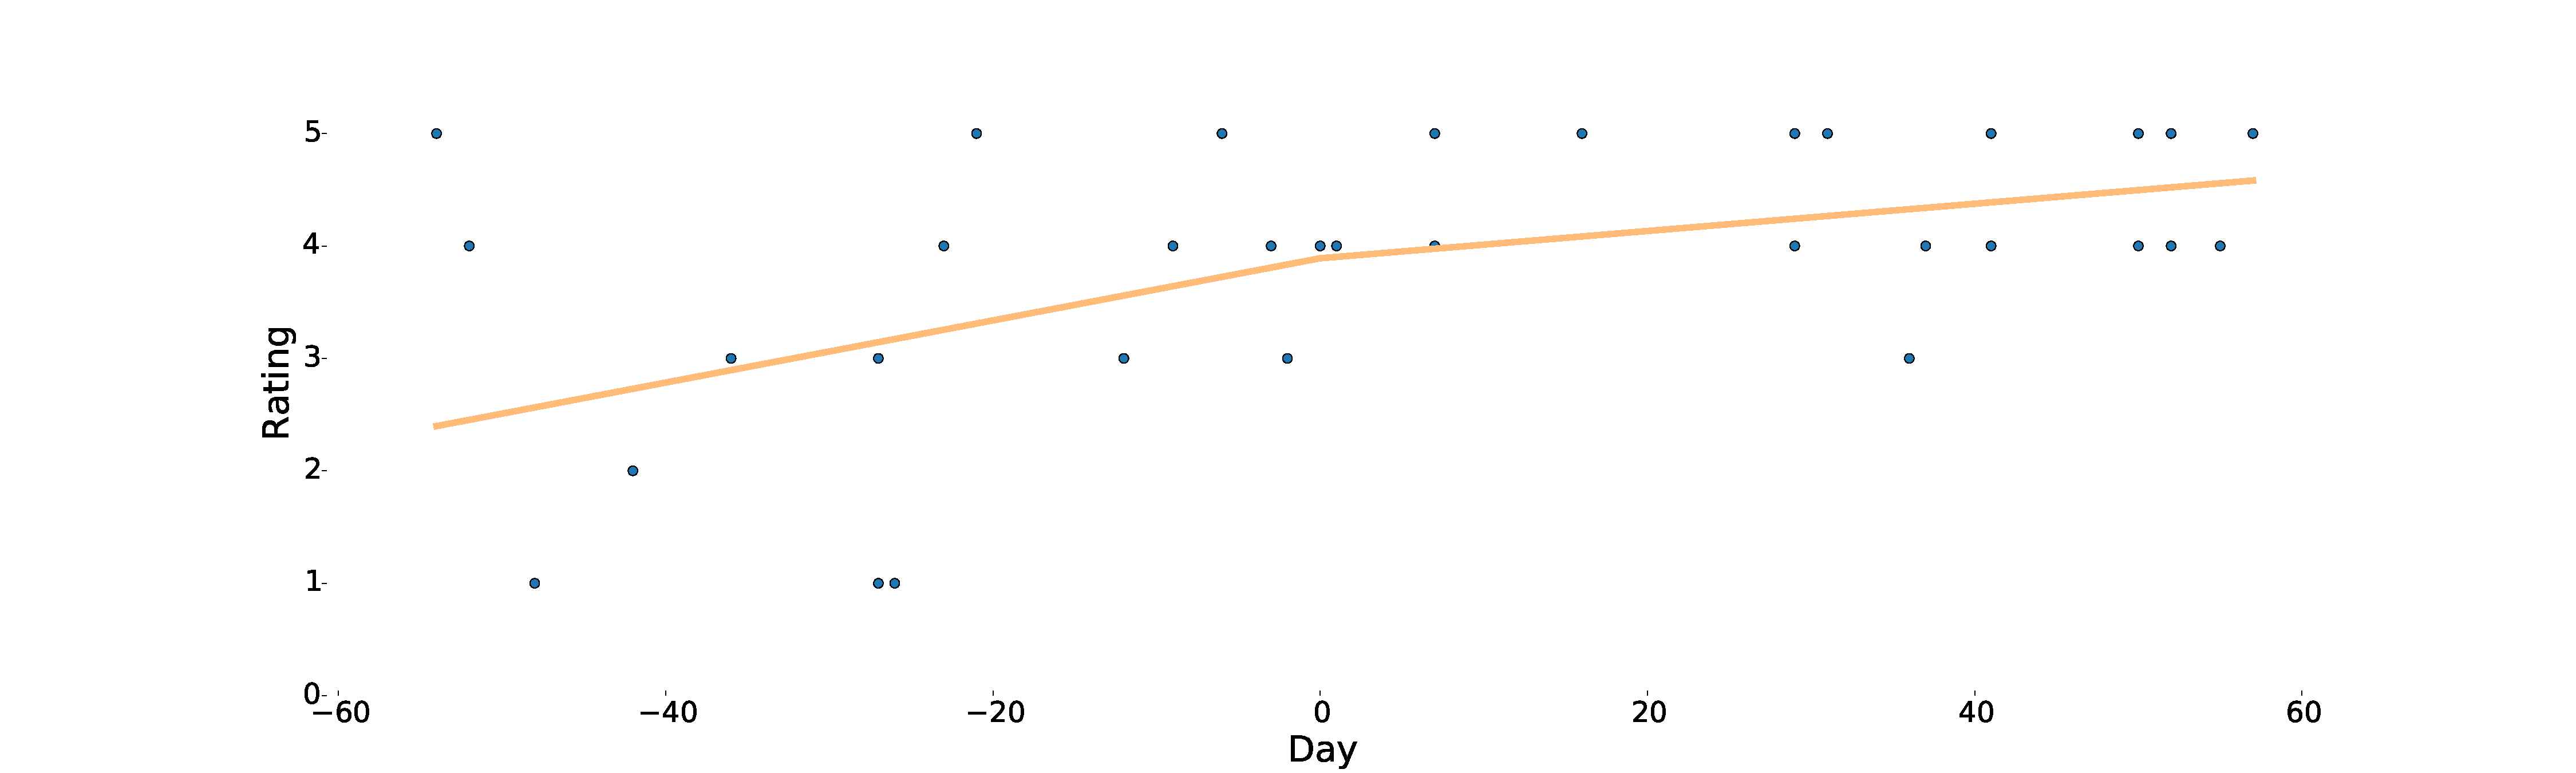
\includegraphics[width=\linewidth]{../trend.pdf}
\captionof{figure}{\color{Green} Example trend analysis for a pair of businesses}
\end{center}


\subsection*{General Trend Analysis}
\textbf{\textit{Hypothesis}} : The exact opening date is not known and since prediction is noisy, the trend analysis might fail. The general trends of the existing businesses around a rough estimate of the opening time of a new business may reflect (with less noise compared to the trend analysis) the impact of the new business on them.\\
\textbf{\textit{Proxy}} : Fit a single line for the ratings of a business around the estimated opening date of a newly opened business in the neighborhood. Determine if the business has an increasing or a decreasing trend based on the slope of the line.\\
\textbf{\textit{Expected results}} : The general trends of the existing businesses around the launching date of a new business in the neighborhood may be predicted using the attributes of the existing businesses and the new business. 

\begin{center}
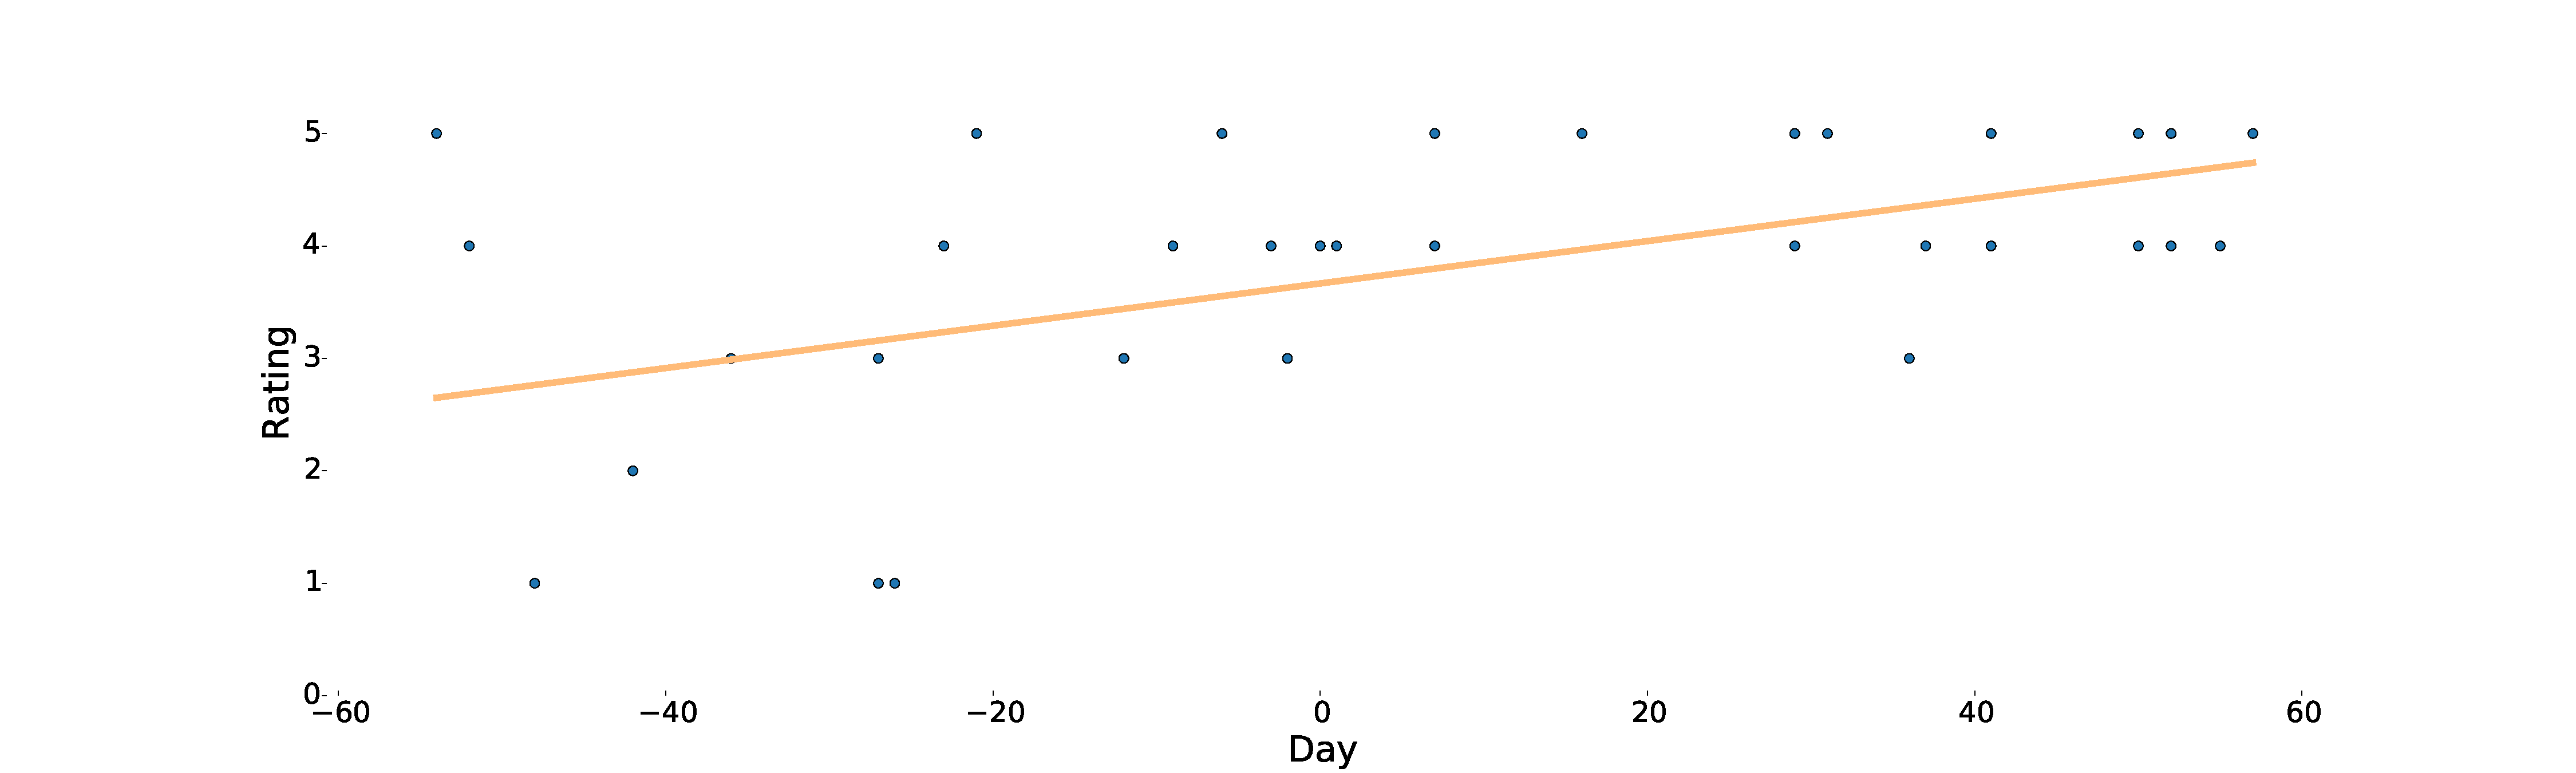
\includegraphics[width=\linewidth]{../gen_trend.pdf}
\captionof{figure}{\color{Green} Example general trend analysis for a pair of businesses}
\end{center}

\subsection*{Correlation Analysis}
\textbf{\textit{Hypothesis}} : None of the previous approaches provided an adequate metric.
For our last model we opted to use a correlation metric which reflects the relationship of two businesses over a long period of time.\\
\textbf{\textit{Proxy}} : Compute the correlation of ratings over time.\\
\textbf{\textit{Expected results}} : The correlation can be predicted using the attributes of the existing businesses and the new business. 

\begin{center}
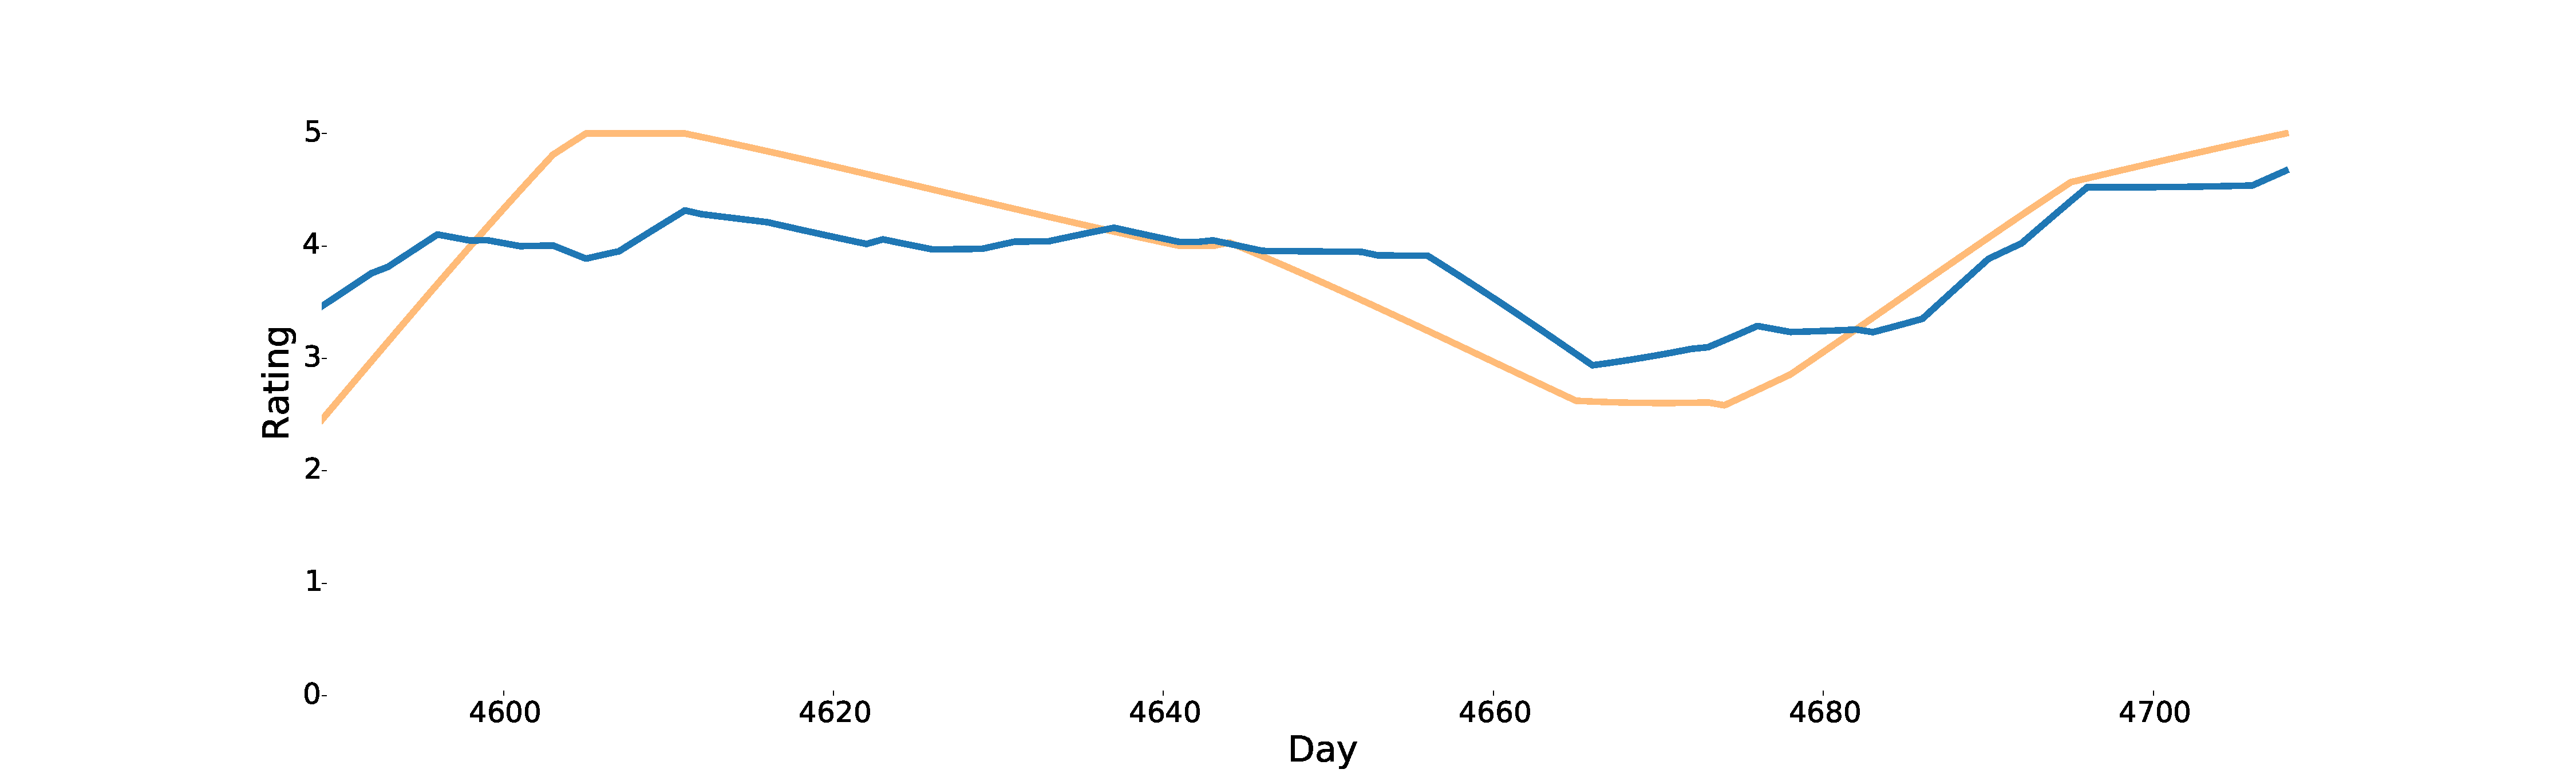
\includegraphics[width=\linewidth]{../corr.pdf}
\captionof{figure}{\color{Green} Example of correlation analysis for a pair of businesses}
\end{center}

%----------------------------------------------------------------------------------------
%	RESULTS 
%----------------------------------------------------------------------------------------

\section*{Results}
%
The following table contains the mean training score and the 10-fold cross-validation score for predictions in a single cluster.
The cluster consists of 147 businesses which corresponds to 10730 pairings.
We did two types of experiments: (a) classification of positive vs. non-positive outcomes for all models and (b) classification of significant vs. insignificant outcomes (absolute value bigger than a certain threshold) for all models.

\begin{table}[H]
\small
% Please add the following required packages to your document preamble:
% \usepackage{multirow}
\begin{tabular}{@{}llrrrr@{}}
\toprule
                                                              &                     & \multicolumn{2}{c}{sig/insig classif.} & \multicolumn{2}{c}{pos/neg classif.} \\ 
\cmidrule(r){3-4}
\cmidrule(r){5-6}
                                                              &                     & \multicolumn{1}{c}{60 days} & \multicolumn{1}{c}{90 days} & \multicolumn{1}{c}{60 days} & \multicolumn{1}{c}{90 days} \\ \midrule
\multirow{2}{*}{Conditional Mean}  & SVM rbf             &   0.84/0.61   &  0.82/0.60  & 0.84/0.60 &  0.85/0.65  \\
                                        & Logistic Regression & 0.61/0.52  & 0.60/0.52 &  0.56/0.49   &  0.56/0.49   \\ \midrule
\multirow{2}{*}{Trend Analysis}       & SVM rbf             & 0.83/0.62    &  0.82/0.59 & 0.84/0.60 & 0.81/0.58   \\
                                        & Logistic Regression &  0.60/0.55   & 0.58/0.48 &  0.57/0.49  &  0.56/0.51   \\ \midrule
\multirow{2}{*}{General Trend Analysis} & SVM rbf             & 0.84/0.62 & 0.80/0.62 &  0.81/0.60 &  0.83/0.63  \\
                                       & Logistic Regression &  0.59/0.52  & 0.58/0.54  &   0.57/0.49  &   0.58/0.49       \\ \midrule
\multirow{2}{*}{Correlation Analysis}   & SVM rbf             & \multicolumn{2}{c}{0.85/0.81}  & \multicolumn{2}{c}{0.86/0.81} \\
                                        & Logistic Regression & \multicolumn{2}{c}{0.84/0.82}  & \multicolumn{2}{c}{0.86/0.83} \\
\bottomrule
\end{tabular}
\captionof{table}{\color{Green} Training and 10-fold cross-validation score for predictions}
\end{table}

\textit{Note}: We do not present the results for linear, poly and sigmoid kernels because the results were significantly worse than SVM with the rbf kernel.


%

%----------------------------------------------------------------------------------------
%	CONCLUSIONS
%----------------------------------------------------------------------------------------

\color{SaddleBrown} % SaddleBrown color for the conclusions to make them stand out

\section*{Conclusions}
We tried to predict the interaction of two businesses with multiple models.
The quality of our predictions turned out to be relatively low for most models.
Possible reasons are:
\begin{itemize}
\item The rating data is noisy and sparse at the same time. Most businesses don't have ratings every day and the variance of the ratings for a given time period is high.
\item The training score of SVM is high in general but the cross-validation score is low in a lot of cases which may be a hint that SVM is overfitting.
\item For the conditional mean analysis and the trend analysis, we assume that the opening date of the business is close to the first review submitted for the business. This might not always be the case.
\end{itemize}

We achieved good results when predicting correlation and this shows that our approach has merit.
We also observed that SVM generally outperformed logistic regression in cases other than correlation analysis.

\color{DarkSlateGray} % Set the color back to DarkSlateGray for the rest of the content

%----------------------------------------------------------------------------------------
%	FORTHCOMING RESEARCH
%----------------------------------------------------------------------------------------


 %----------------------------------------------------------------------------------------
%	REFERENCES
%----------------------------------------------------------------------------------------

\nocite{*} % Print all references regardless of whether they were cited in the poster or not
\bibliographystyle{plain} % Plain referencing style
\bibliography{sample} % Use the example bibliography file sample.bib

%----------------------------------------------------------------------------------------

\end{multicols}
\end{document}